\documentclass[a4paper,12pt]{article}
\usepackage[utf8]{inputenc}
\usepackage[italian]{babel}
\usepackage{graphicx}
\usepackage{amsmath}
\usepackage{amssymb}
\usepackage{hyperref}
\usepackage{algorithm}
\usepackage{algpseudocode}
\usepackage{csquotes}

\title{Solving the Weighted Feedback Vertex Set Problem using a Hybrid Genetic Algorithm}
\author{Francesco Granata \\ Università di Catania \\ 1000046547}
\date{10 Marzo 2025}

\begin{document}

\maketitle
\newpage
\tableofcontents 
\newpage

\section{Introduzione}
\subsection{Definizione}
Il \textit{Weighted Feedback Vertex Set Problem} (WFVS) è un problema di ottimizzazione combinatoria che consiste nel trovare un sottoinsieme di vertici il cui rimuovimento renda il grafo aciclico, minimizzando la somma dei pesi dei nodi rimossi. 

\subsection{Definizione Formale}
Formalmente, dato un grafo non orientato \( G = (V, E) \), un insieme di vertici di feedback di \( G \) è un sottoinsieme \( S \subseteq V \) di vertici la cui rimozione, insieme a tutti i lati incidenti in \( S \), rende il grafo aciclico, ovvero \( G(V \setminus S, E \setminus S) \) è un grafo aciclico.

Inoltre, sia \( w: V \to \mathbb{R}^{+} \) una funzione peso che associa un valore positivo a ciascun vertice \( v \in V \) in \( G \). Il peso dell'insieme di vertici di feedback \( S \subseteq V \) è la somma dei pesi dei suoi vertici, cioè \( \sum_{v \in S} w(v) \).

Risolvere il problema del \textit{Weighted Feedback Vertex Set} richiede di trovare un insieme \( S \) di minimo peso, ovvero:

\begin{equation}
\min_{S} \sum_{v \in S} w(v)
\end{equation}

\subsection{Complessità Computazionale}
Il \textit{WFVS} è un problema \textit{NP-Hard}, quindi è impossibile trovare una soluzione che di per certo è ottima in tempo polinomiale:
Per questo motivo siamo costretti a utilizzare tecniche euristiche e metaeuristiche che approssimano la soluzione in tempi polinomiali.

\subsection{Applicazioni}
Questo problema ha importanti applicazioni:
\begin{itemize}
    \item \textbf{Teoria dei Grafi}: Rimuove cicli per ottimizzare reti o risolvere dipendenze circolari.
    \item \textbf{Intelligenza Artificiale}: Garantisce che reti bayesiane siano acicliche, migliorando algoritmi di apprendimento.
    \item \textbf{Biologia Computazionale}: Analizza reti metaboliche e interazioni proteiche, identificando nodi chiave per interrompere cicli.
    \item \textbf{Ingegneria dei Sistemi}: Stabilizza sistemi di controllo e ottimizza processi industriali rimuovendo cicli.
    \item \textbf{Informatica Teorica}: È un problema NP-difficile, studiato per sviluppare algoritmi di approssimazione euristici.
    \item \textbf{Applicazioni Pratiche}: Migliora sistemi di raccomandazione e gestione di progetti eliminando conflitti ciclici.
\end{itemize}



\section{Algoritmo Sviluppato}
Per affrontare questo problema, è stato sviluppato un Algoritmo Genetico Ibrido \textbf{(HGA - Hybrid Genetic Algorithm)}, che combina le caratteristiche dei \textbf{Genetic Algorithms (GA)} con una fase di \textbf{ricerca locale} per migliorare la qualità delle soluzioni trovate. Gli Algoritmi Genetici sono ispirati alla selezione naturale e si basano su operatori di selezione, crossover e mutazione per esplorare lo spazio delle soluzioni. Tuttavia, una pura strategia evolutiva potrebbe soffrire di convergenza prematura o stagnazione su ottimi locali.

L'approccio ibrido integra quindi un meccanismo di \textbf{local search} che affina le soluzioni generate dal processo evolutivo, migliorando progressivamente la qualità dei candidati senza perdere la diversità della popolazione. Grazie a questa combinazione, l'algoritmo sfrutta la capacità esplorativa degli Algoritmi Genetici e la forza di intensificazione della ricerca locale, garantendo un compromesso efficace tra esplorazione ed exploitation dello spazio delle soluzioni.

In generale le fasi di questo algoritmo sono riassunte in questi punti:

\begin{itemize}
    \item \textbf{Inizializzazione della popolazione}: Viene generata una popolazione iniziale di soluzioni casuali.
    \item \textbf{Fitness}: Per ogni individuo della popolazione, viene calcolata la sua funzione di valutazione (fitness) che potrebbe cambiare in base al problema.
    \item \textbf{Selezione dei genitori}: Viene utilizzata una strategia di selezione che prende un sottoinsieme della popolazione. Gli elementi selezionati saranno i padri della nuova popolazione. La scelta è basata sulla fitness.
    \item \textbf{Crossover}: Gli individui selezionati subiscono un crossover, che combina le caratteristiche dei genitori per generare nuovi individui (figli).
    \item \textbf{Mutazione}: Con una certa probabilità avvengono mutazioni alla popolazione. Serve a mantenere diversità nella popolazione e previene una convergenza prematura verso i minimi locali.
    \item \textbf{Ricerca locale}: Attraverso una ricerca locale si cerca di migliorare le soluzioni trovate per convergere prima verso la giusta soluzione.
    \item \textbf{Aggiornamento della popolazione}: Si prende la nuova popolazione creata e si integra con quella vecchia nel modo più opportuno.
    \item \textbf{Criterio di terminazione}: Un ciclo dei punti sopra elencati viene fatto fin quando, secondo un certo criterio di terminazione, viene interrotto e si ritorna la soluzione
\end{itemize}

Nel seguito del documento, verranno approfonditi i dettagli dell'implementazione, le scelte progettuali e le metodologie utilizzate per garantire prestazioni ottimali nell'identificazione dell'insieme di vertici di feedback a peso minimo.

\section{Implementazione}
L'algoritmo è stato implementato in Python, utilizzando la libreria NetworkX per la gestione dei grafi. Il codice è strutturato in modo modulare.
Ecco un approfondimento sul come è stato deciso di sviluppare l'HGA.

\subsection{Inizializzazione della popolazione}
Crea una popolazione iniziale di soluzioni random.
la popolazione è composta da vettori binari lunghi quanto il numero dei nodi del grafo
su ogni vettore creato chiamiamo una local search in modo da ottimizzarlo subito. 

La grandezza della popolazione scelta è: 
\begin{verbatim}
pop_size = 100
\end{verbatim}
La scelta è derivata dal non voler utilizzare una grandezza della popolazione troppo bassa (50) ma comunque tenersi sul medio-basso per limitare i tempi di esecuzione.
\begin{algorithm}[H]
\caption{initialize population}
\begin{algorithmic}[1]
\Require pop\_size, num\_nodes, graph
\Ensure population
\State population $\leftarrow$ []
\For{$i = 1$ to pop\_size}
    \State solution $\leftarrow$ vettore binario casuale di lunghezza num\_nodes
    \State solution $\leftarrow$ \textsc{Local\_Search}(solution, graph)
    \State population.append(solution)
\EndFor
\State \Return population
\end{algorithmic}
\end{algorithm}

\subsection{Fitness}
La Fitness da calcolare per il problema del WFVS è la somma dei pesi dei vertici selezionati.
\begin{itemize}
    \item Prende la soluzione inviata e crea un sottografo senza i nodi selezionati.
    \item Ritorna la somma dei pesi della soluzione.
    \item Se il grafo non è aciclico tornerà la fitness della soluzione con una penitenza calibrata in base al numero di cicli.
    Questo per penalizzare le soluzioni che hanno più cicli rispetto ad altre.
\end{itemize}
\begin{algorithm}[H]
\caption{fitness}
\begin{algorithmic}[1]
\Require solution, node\_weights, graph
\Ensure fitness + pensalità in caso di cicli
\State Incrementa il contatore delle valutazioni $evaluation\_count$
\State Determina l'insieme dei nodi da rimuovere: 
\State \quad $nodes\_to\_remove \gets \{ v \mid v \in V, \mathit{solution}[v] = 1 \}$
\State Crea il sottografo senza i nodi selezionati: $subgraph \gets graph - nodes\_to\_remove$
\State Conta il numero di cicli nel sottografo: $num\_cycles \gets$ numero di cicli in $subgraph$
\State Calcola il valore della fitness: 
\State \quad $fitness \gets \sum_{v \in nodes\_to\_remove} node\_weights[v] + 10000 \cdot num\_cycles$
\Return $fitness$
\end{algorithmic}
\end{algorithm}

\subsection{Selezione dei genitori}
Per selezionare i genitori destinati alla riproduzione, è stata utilizzata la \textit{k-Tournament Selection}, che funziona come segue:
\begin{itemize}
    \item Si selezionano casualmente k individui dalla popolazione.
    \item Si confrontano i valori di fitness e si sceglie il migliore come genitore.
\end{itemize}
Come k si è scelto di utilizzare:
\begin{verbatim}
k = 5
\end{verbatim}
per trovare più velocemente buone soluzioni.
\begin{algorithm}
\caption{tournament selection}
\begin{algorithmic}[1]
\Require population, fitnesses (fitness di tutta la popolazione)
\Ensure soluzione vincente
\State Seleziona casualmente $k$ individui dalla popolazione
\State Estrai i corrispondenti valori di fitness
\State Determina il miglior individuo tra i $k$ selezionati (quello con fitness minima)
\State \Return soluzione vincente
\end{algorithmic}
\end{algorithm}

\subsection{Crossover}
Come Crossover è stato utilizzato un \textit{Three-Point Crossover} il cui funzionamento è:
\begin{itemize}
    \item Si selezionano tre punti casuali nei cromosomi dei genitori.
    \item Si ordinano i punti
    \item Vengono scambiati i bit dei parent tra il punto 1 e il punto 2 e quelli dopo il punto 3
    \item I due nuovi vettori saranno i child da tornare.
\end{itemize}
\begin{algorithm}
\caption{Crossover}
\begin{algorithmic}[1]
\Require parent1, parent2
\Ensure child1, child2
\State Seleziona tre punti distinti casuali e ordinali in ordine crescente
\State Copia $\mathit{parent1}$ in $\mathit{child1}$ e $\mathit{parent2}$ in $\mathit{child2}$
\State Scambia i segmenti tra il primo e il secondo punto tra i genitori
\State Scambia i segmenti dopo il terzo punto tra i genitori
\State \Return $\mathit{child1}$, $\mathit{child2}$
\end{algorithmic}
\end{algorithm}

\subsection{Mutazione}
Per mantenere la diversità nella popolazione, si applica una mutazione con probabilità $P_m$.

Come $P_m$ si è scelto di utilizzare:
\begin{verbatim}
    mutation_rate = 0.01
\end{verbatim}
per evitare di cadere in ottimi locali.
\begin{algorithm}[H]
\caption{mutate}
\begin{algorithmic}[1]
\Require Una soluzione $\mathit{solution}$ (array di bit) e un tasso di mutazione $\mathit{mutation\_rate}$
\Ensure Una nuova soluzione mutata
\State Genera una maschera di mutazione casuale, dove ogni bit ha probabilità $\mathit{mutation\_rate}$ di essere selezionato
\State Inizializza una lista vuota per la soluzione mutata
\For{ogni bit nella soluzione originale}
    \If{il bit è stato selezionato dalla maschera di mutazione}
        \State Inverti il bit (da 0 a 1 o da 1 a 0) e aggiungilo alla soluzione mutata
    \Else
        \State Aggiungi il bit originale alla soluzione mutata
    \EndIf
\EndFor
\State \Return la soluzione mutata
\end{algorithmic}
\end{algorithm}

\subsection{Ricerca locale}
Viene implementata una ricerca locale di tipo greedy per ottimizzare una soluzione rappresentata come un array di bit

L'obiettivo è rimuovere nodi selezionati dalla soluzione, mantenendo la proprietà di aciclicità del grafo. Per evitare un numero eccessivo di iterazioni, viene utilizzato un limite massimo di iterazioni (\textit{max\_iter}).

Si è scelto come valore di \textit{max\_iter}:
\begin{verbatim}
    max_iter = 30
\end{verbatim}
\begin{algorithm}[H]
\caption{local\_search}
\begin{algorithmic}[1]
\Require Una soluzione $\mathit{solution}$ (array di bit) e un grafo $\mathit{graph}$
\Ensure Una soluzione migliorata $\mathit{improved\_solution}$
\State Imposta un limite massimo di iterazioni $\mathit{max\_iter} \gets 30$
\State Inizializza un contatore $\mathit{count} \gets 0$
\State Copia la soluzione originale in $\mathit{improved\_solution}$
\For{ogni bit nella soluzione originale}
    \If{il bit è uguale a $1$}
        \State Imposta il bit a $0$ in $\mathit{improved\_solution}$
        \If{il grafo $\mathit{graph}$ non è aciclico con $\mathit{improved\_solution}$}
            \State Ripristina il bit a $1$ in $\mathit{improved\_solution}$
        \EndIf
    \EndIf
    \State Incrementa $\mathit{count}$ di $1$
    \If{$\mathit{count} \geq \mathit{max\_iter}$}
        \State Interrompi il ciclo
    \EndIf
\EndFor
\State \Return $\mathit{improved\_solution}$
\end{algorithmic}
\end{algorithm}

\subsection{Aggiornamento della popolazione}
Per aggiornare in modo opportuno la popolazione si è fatto nel seguente modo:
\begin{itemize}
    \item Viene aggiunta la nuova popolazione a quella vecchia
    \item Si ordina rispetto alla fitness
    \item Si riduce il vettore della popolazione a \textit{pop\_size}
\end{itemize}

\subsection{Criterio d'arresto}
Si è impostato il criterio di arresto a:
\begin{verbatim}
    generations = 1001
\end{verbatim}

\section{Analisi Sperimentale}
\subsection{Protocollo Sperimentale}
Sono stati condotti esperimenti su un totale di 30 istanze del problema, con grafi non orientati di tipi e dimensioni variabili. 

6 grafi diversi, per ognuno 5 istanze in cui varia la funzione peso \textit{w}.
In particolare questi 6 grafi sono grafi con 2 topologie diverse: 3 a griglia e 3 casuali.

Il protocollo utilizzato:
\begin{itemize}
    \item Su ogni istanza sono state fatte 10 Run diverse per trovare la soluzione minima.
    \item I risultati di ogni istanza sono stati inseriti in un dataframe creato con la libreria Python "\textit{Pandas}", poi salvati in un file \textit{.xlsx}.
    \item Per ogni grafo si calcola la media, la deviazione standard e la media del numero di valutazioni della fitness sui minimi delle 5 istanze.
\end{itemize}

\subsection{Risultati Sperimentali}
La seguente tabella contiene i risultati sperimentali raccolti seguendo il protocollo precedentemente descritto.

\begin{table}[H]
\centering
\begin{tabular}{|c|c|c|c|}
\hline
Tipo Grafo & Media & Dev. Std. & Media Valutazioni Fitness \\
\hline
\textbf{Grid\_5\_5} & 199,8 & 21,8 & 201301.0 \\
\textbf{Grid\_7\_7} & 254,8 & 5,8 & 201301.0 \\
\textbf{Grid\_9\_9} & 1184,4 & 134,9 & 201301.0 \\
\textbf{Rand\_100\_3069} & 1139,6 & 19,8 & 201301.0 \\
\textbf{Rand\_100\_841} & 1794,2 & 127,9 & 201301.0 \\
\textbf{Rand\_200\_3184} & 5366,0 & 867,2  & 201301.0 \\
\hline
\end{tabular}
\caption{Risultati sperimentali.}
\end{table}

\subsection{Grafi e Grafici}
\begin{figure}[H]
\centering
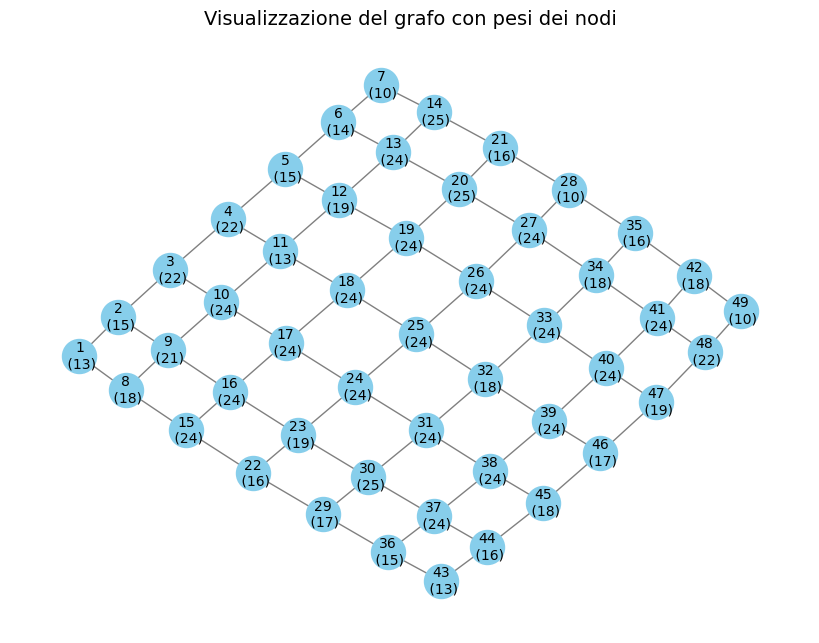
\includegraphics[width=0.7\textwidth]{img/grafo_grid_7_7.png}
\caption{Grafo di tipo Grid\_7\_7 (INPUT)}
\end{figure}
\begin{figure}[H]
\centering
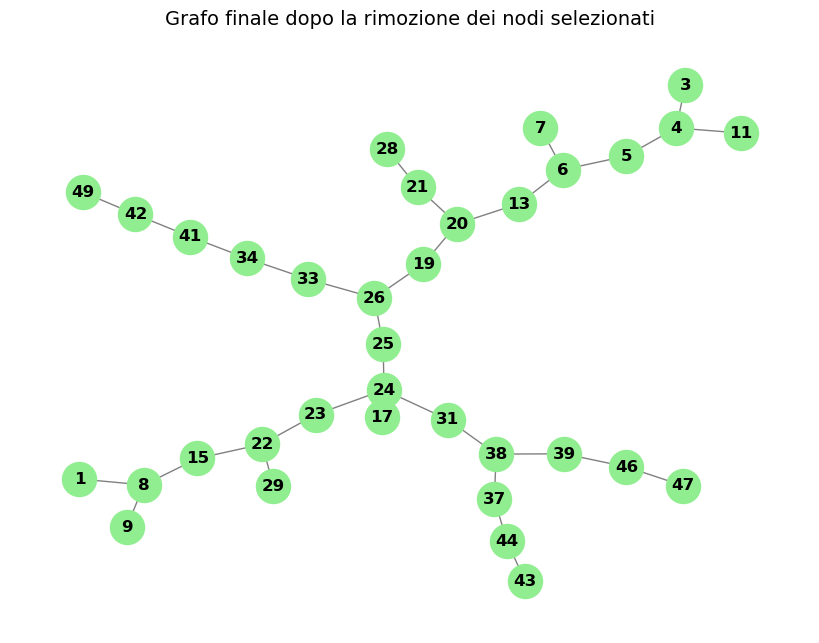
\includegraphics[width=0.7\textwidth]{img/grafoAciclico_grid_7_7.png}
\caption{Grafo di tipo Grid\_7\_7 (OUTPUT)}
\end{figure}
\begin{figure}[H]
\centering
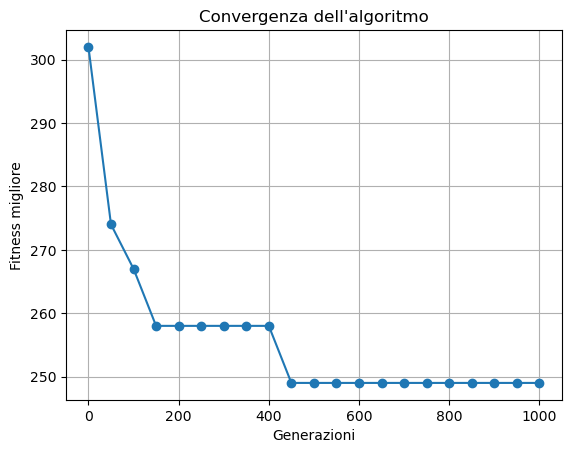
\includegraphics[width=0.7\textwidth]{img/convergenza_grid_7_7.png}
\caption{Grafo di tipo Grid\_7\_7 (CONVERGENZA FITNESS)}
\end{figure}

\section{Conclusioni}
In questo lavoro abbiamo affrontato il \textbf{Weighted Feedback Vertex Set Problem (WFVS)}, un problema \textbf{NP-Hard} con numerose applicazioni pratiche, sviluppando e testando un \textbf{Hybrid Genetic Algorithm (HGA)} per trovare soluzioni approssimate di alta qualità.

Possiamo dire che:
\begin{itemize}
    \item L'analisi delle diverse istanze ha evidenziato come la topologia del grafo e la distribuzione dei pesi influiscano sulla difficoltà del problema, mostrando che l'HGA si adatta bene a scenari diversi. Inoltre, il protocollo sperimentale ha permesso di valutare in modo oggettivo le performance dell'algoritmo, evidenziando la stabilità dei risultati ottenuti su più esecuzioni indipendenti.
    \item Si nota che per i grafi più semplici l'algoritmo converge dopo poche iterazioni, mentre per istanze più grandi sono necessarie tutte e 1000 le generazioni.
    \item Il compromesso tra qualità delle soluzioni e tempo di esecuzione è pressochè buono.
    \item Bilancia esplorazione e sfruttamento, combinando la diversità della ricerca genetica con la precisione della ricerca locale.
\end{itemize}

Nonostante i risultati promettenti ottenuti con l'HGA, vi sono diversi aspetti che potrebbero essere migliorati per ottimizzare ulteriormente l'algoritmo:
\begin{itemize}
    \item \textbf{Ottimizzazione dei parametri}: una ricerca automatica dei parametri tramite tecniche come l'ottimizzazione bayesiana o l'evoluzione differenziale potrebbe migliorare le prestazioni.
    \item \textbf{Strategie avanzate di mutazione e crossover}: l'introduzione di operatori adattivi o basati su euristiche specifiche per il WFVS potrebbe portare a una convergenza più rapida e soluzioni di qualità superiore.
    \item \textbf{Miglioramento Local Search}: implementare un altro tipo di local search potrebbe rendere l'algoritmo più veloce o performante.
    \item \textbf{Ibridazione con altri metodi}: combinare l'HGA con tecniche come il simulated annealing o la programmazione matematica potrebbe aumentare l'efficienza nell'esplorare lo spazio delle soluzioni.
    \item \textbf{Parallelizzazione}: implementare il calcolo parallelo per la valutazione della fitness o per l'esecuzione delle ricerche locali permetterebbe di ridurre significativamente i tempi di esecuzione, rendendo l'algoritmo applicabile a istanze ancora più grandi.
\end{itemize}

L'algoritmo sviluppato si è dimostrato un metodo efficace per affrontare il WFVS, fornendo soluzioni competitive in tempi ragionevoli. L'analisi sperimentale ha confermato la robustezza dell'approccio, bilanciando esplorazione e sfruttamento per migliorare progressivamente le soluzioni. Grazie alla sua flessibilità, l'HGA potrebbe essere ulteriormente adattato e migliorato, aprendo la strada a nuove ricerche nel campo dell'ottimizzazione combinatoria.

\newpage

\bibliographystyle{plain}  % Stile della bibliografia (puoi cambiare, es: alpha, apa, ieee)
\bibliography{bibliografia}
\nocite{*}

\end{document}